\documentclass[11pt]{article}
\usepackage{fontspec}
\usepackage[margin=1in,left=1.5in,includefoot]{geometry}
\setmainfont[Ligatures=TeX]{Linux Libertine O}
% Graphic
\usepackage{graphicx}
\usepackage{float}

% Hyperlinks
\usepackage{hyperref}

% Header and footer
\usepackage{fancyhdr}
\pagestyle{fancy}
\fancyfoot{}
\fancyhead[LE,RO]{\bfseries\thepage}
\setlength{\headheight}{15pt}

% Quotes character
\usepackage[utf8]{inputenc}

% color links
\usepackage{color}  
\usepackage{hyperref}
\hypersetup{
    colorlinks=true, %set true if you want colored links
    linktoc=all,     %set to all if you want both sections and subsections linked
    linkcolor=black,  %choose some color if you want links to stand out
    urlcolor=blue
}

\begin{document}
\begin{titlepage}
	\begin{center}

\includegraphics[width=0.6\textwidth]{images/bordeaux.png}\\[1cm]


{\large Report}\\[0.5cm]	
	
	\line(1,0){400}\\[0.2in]
	\huge{\bfseries Deep Learning}\\
	\line(1,0){400}\\[1.5cm]
	
	\noindent	
	
	\begin{minipage}[t]{0.4\textwidth}
		\begin{flushleft} \large
    	\emph{Author:}\\%
    	Manh Tu \textsc{Vu}
		\end{flushleft}
	\end{minipage}
	\begin{minipage}[t]{0.4\textwidth}
  		\begin{flushright} \large
    		\emph{Supervisor:} \\
    		Marie\textsc{Beurton-Aimar}
  		\end{flushright}
	\end{minipage}
	
	\vfill

% Bottom of the page
{\large \today}
	\end{center}
\end{titlepage}

% Front matter
\pagenumbering{arabic}

% Table content
\tableofcontents
\thispagestyle{empty}
\clearpage

% List of figures 
%\listoffigures
%\clearpage

\section*{Abstract}
In this project, we use Deep Learning method to automatic classify images from \href{https://heobs.org}{https://heobs.org} into 4 classes, include:
\begin{itemize}
\item Heritage
\item Beings
\item Scenery/Landscape
\item Other
\end{itemize}

\section{Introduction}
\section{Preparing images}
\subsection{Fetch all images}
The entire image dataset described on the text file "photos.txt" line by line. Each line include the image id and image description. 
\begin{verbatim}
	 5a36f382-dbdf-11e6-95fd-d746d863c3eb | Những người ăn xin  | vie
	 5a36f382-dbdf-11e6-95fd-d746d863c3eb | Mendiants  | fra
	 17be8122-dbe0-11e6-860c-5fea02802d0a | Chợ Cũ (3) | vie
	 17be8122-dbe0-11e6-860c-5fea02802d0a | Vieux marché (3) | fra
	 400286c8-dbe1-11e6-bb4d-ff975c68de04 | Ngân hàng Đông Dương  | vie
	 400286c8-dbe1-11e6-bb4d-ff975c68de04 | La Banque de l’Indochine  | fra
\end{verbatim}
In order to get the image dataset, we have to fetch each images one by one by join the image id with heobs cdn url \href{https://cdn.heobs.org/photo/}{https://cdn.heobs.org/photo/}. For example, with the first line in the record above, we have the following URL: 
\begin{verbatim}
 https://cdn.heobs.org/photo/5a36f382-dbdf-11e6-95fd-d746d863c3eb
\end{verbatim}
Finally, we write a smaill python script to automatic read this text file \& download images one by one.

\subsection{Remove dupplicate images}
In the "photos.txt", some image have two languages and then, it consume two lines. As the record above, we have 6 lines but 

\begin{figure}[H]
\centering
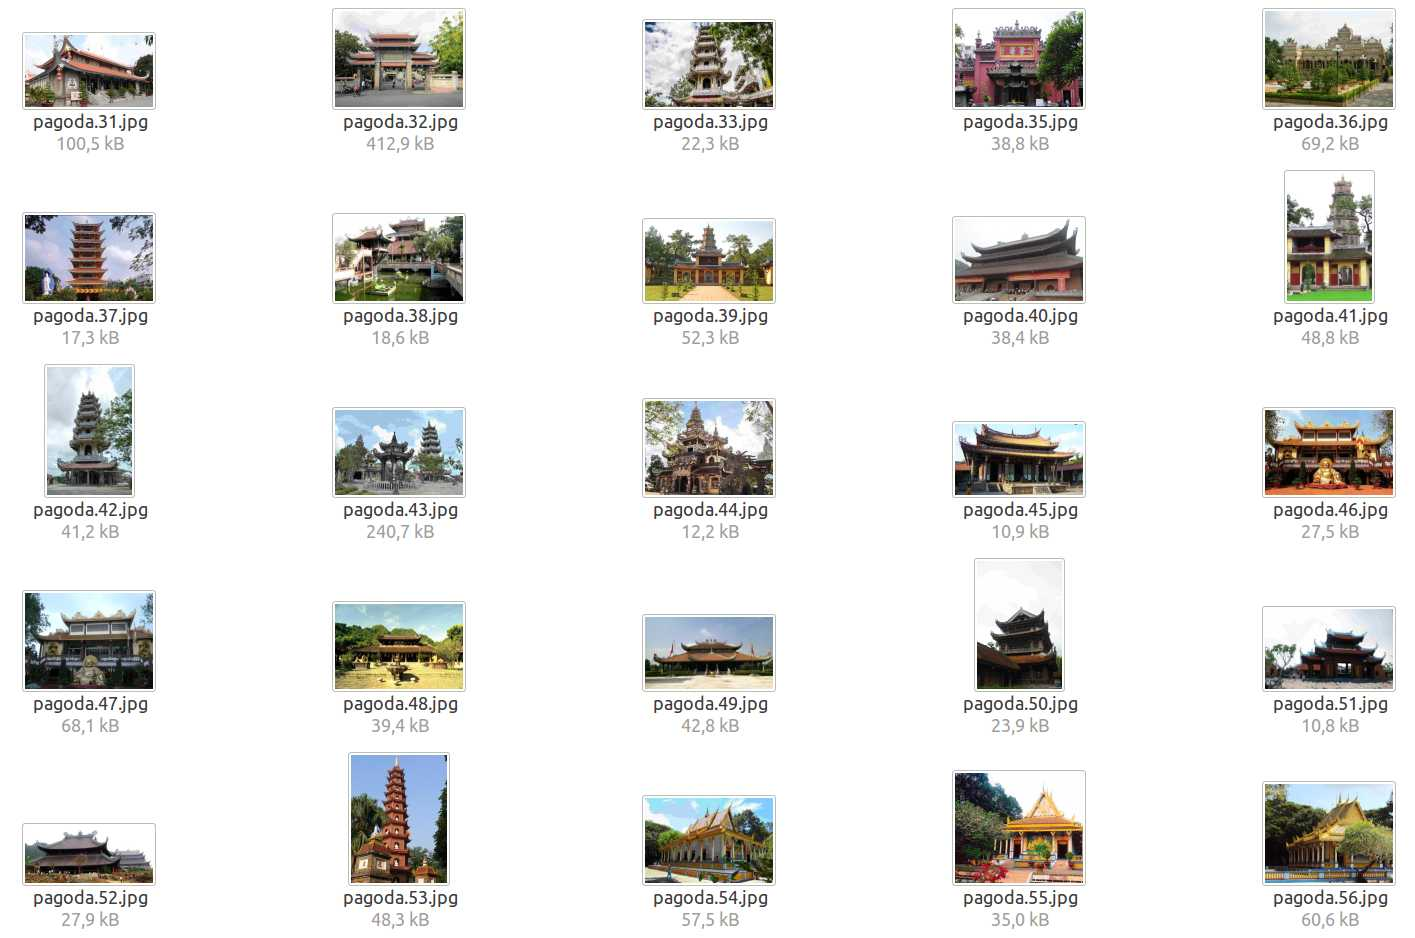
\includegraphics[width=1\textwidth]{images/sample.jpg}
\caption{Sample pagoda images from our training dataset}
\label{fig:samplepagoda}
\end{figure}
Our training set contains 500 images of pagoda, while the test dataset contains 20 images. The average size for these images is around 350x500.

\section{Our solution}
\subsection{Hardware}
We hire Amazon Web Services, create G2 instance:
\begin{center}
\begin{tabular}{| c | c | c | c | c |}
\hline
 Model & GPUs & vCPU & Mem (GiB) & SSD Storage (GB) \\ 
\hline
 g2.2xlarge & 1 & 8 & 15 & 1 x 60  \\
\hline
\end{tabular}
\end{center}

\subsection{Method using}

\section{Result and Analysis}




\bibliographystyle{plain}
\bibliography{bibfile}
\end{document}